%
% LaTeX Report Assignment 4
% Applied Programming Lab EE2703
% Ayush Jamdar EE20B018 
%


\documentclass[11pt, a4paper]{article}
\usepackage{graphicx}
\usepackage{amsmath}
\usepackage{listings}
\usepackage[]{courier}
%\usepackage{hyperref}


\title{Assignment 6: The Laplace Transform} % Title

\author{Ayush Jamdar EE20B018} % Author name

\date{\today} % Date for the report
\begin{document}		
		
\maketitle % Insert the title, author and date
\section{Aim}
The goal is to analyse Linear Time-Invariant Systems with numerical methods in python. The \texttt{scipy.signal} 
module is used as a powerful tool to simplify and solve rational functions, transfer functions and Laplace Transforms. The table in the assignment manual explains the use of all functions of this module that would be needed.

\section{The Assignment}
\subsection{Laplace Transform}
The Laplace Transform of $f(t)=\cos(1.5t)e^{-0.5t}u(t)$ is given by $$F(s)=\frac{s+0.5}{(s+0.5)^2+2.25}$$
From a system point of view, $f(t)$ is the input to the system and $x(t)$ is the output. To find $x(t)$, I need to solve for the time response of a spring governed by the equation $$\frac{d^2x}{dx^2}+2.25x=f(t)$$
Given initial conditions $x(0)=0$ and $\dot x(0)=0$. These initial conditions play a crucial role when taking the Laplace transform of derivatives (unilateral transforms). The way is to convert the above differential equation into a Laplace polynomial, get $X(s)$ and take the Laplace inverse. The \texttt{sp.impulse} function does this.

\begin{verbatim}
F1_s = sp.lti([1, 0.5], [1, 1, 2.5])
X1_s = sp.lti([1, 0.5], np.polymul([1, 0, 2.25],
 [1, 1, 2.5]))
t, x1 = sp.impulse(X1_s, None, np.linspace(0, 50, 1000))
# this gives the inverse laplace transform
plt.plot(t, x1)
plt.title("Time Response")
plt.xlabel(r'time $\rightarrow$')
plt.ylabel(r'x(t) $\rightarrow$')
plt.show()
\end{verbatim}

The time response is plotted in Figure 1.

\begin{figure}[!tbh]
   	\centering
  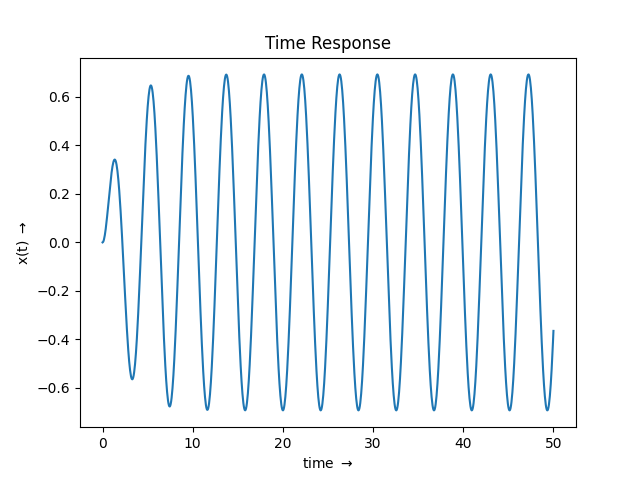
\includegraphics[scale=0.5]{Q1.png} 
    \caption{$x(t)$} 	
    \label{time response}
   \end{figure} 
   
\subsection{Question 2}
The question wants one to do the same computation for $x(t)$, just with a decay of 0.005 instead. A similar code gives the output shown in Figure 2. 

\begin{figure}[!tbh]
   	\centering
  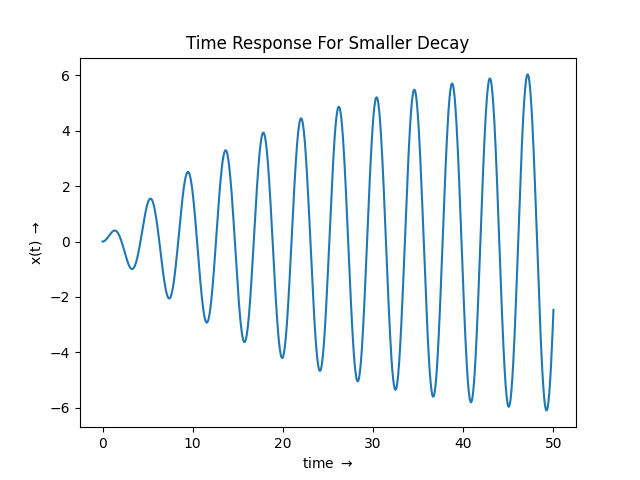
\includegraphics[scale=0.5]{Q2.png} 
    \caption{$x(t)$ at decay 0.05} 	
    \label{time response 2}
   \end{figure} 
   
\subsection{Question 3: The LTI System}
For this input-output nomenclature, the transfer function is given by $X(s)/F(s)$. In a loop, I take four frequencies of $f(t)$ from 1.4 to 1.6 and plot the corresponding input output plots. \texttt{sp.lti(Num,Den} defines the rational polynomial transfer function. \texttt{sp.lsim} takes the input signal and the transfer function to give the input signal in time domain.
 
\begin{verbatim}
freq = np.linspace(1.4,1.6,5)
for f in freq:
    F_s = sp.lti([1, 0.5], [1, 0.1, (f**2)+0.0025])
    X_s = sp.lti([1, 0.5], np.polymul([1, 0, 2.25], 
    [1, 0.1, (f**2)+0.0025]))
    H_s = sp.lti([1],[1,0,2.25])  
    # Obtain the transfer function X(s)/F(s)
    time_interval = np.linspace(0,50,1000)
    f_t = np.cos(f*time_interval)*(np.exp(-0.05*time_interval))
    t,x_t,svec = sp.lsim(H_s,f_t,time_interval)
    plt.subplot(1,2,1)
    plt.plot(time_interval, x_t,label='Output function')
    plt.xlabel(r'time $\rightarrow$')
    plt.ylabel(r'x(t) $\rightarrow$')
    plt.title('x(t) output')
    plt.subplot(1,2,2)
    plt.plot(time_interval,f_t,'red',label='Input function')
    plt.legend()
    plt.ylabel('f(t)')
    plt.title("f(t) at frequency {}".format(round(f, 2)))
    plt.show()

\end{verbatim}

The five outputs are shown in Figures 3-7. The differential equation tells that 1.5 is the natural frequency of the LTI system. Hence the maximum output amplitude is obtained at 1.5. The max amplitude increases as we move towards 1.5 and reduces after that. 

\begin{figure}[!tbh]
   	\centering
  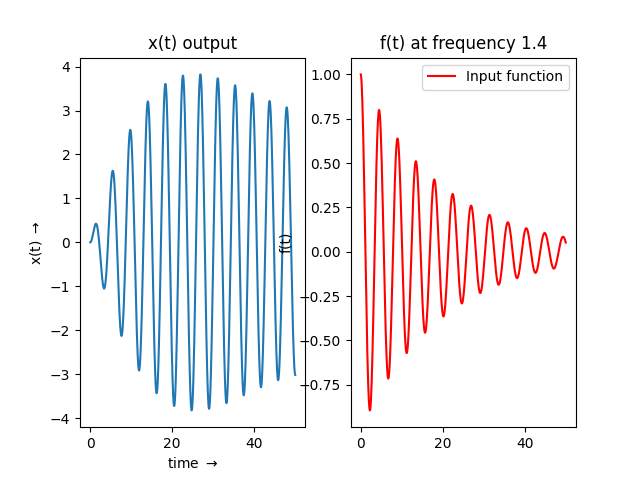
\includegraphics[scale=0.5]{Q3-1.png} 
    \caption{Question 3} 	
    \label{time response q3.1}
   \end{figure} 
   
\begin{figure}[!tbh]
   	\centering
  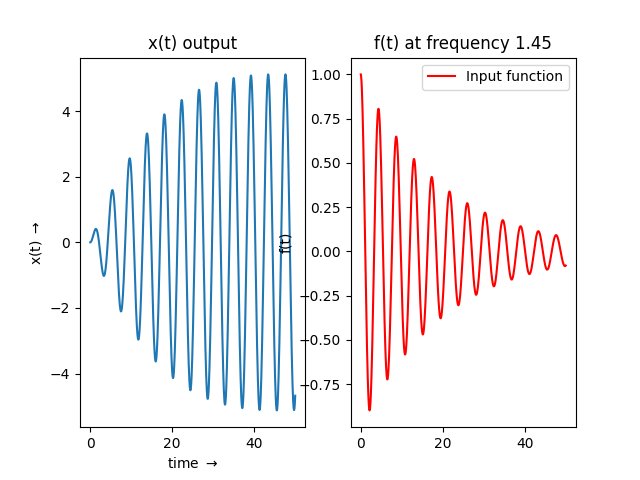
\includegraphics[scale=0.5]{Q3-2.png} 
    \caption{Question 3} 	
    \label{time response q3.2}
   \end{figure} 

\begin{figure}[!tbh]
   	\centering
  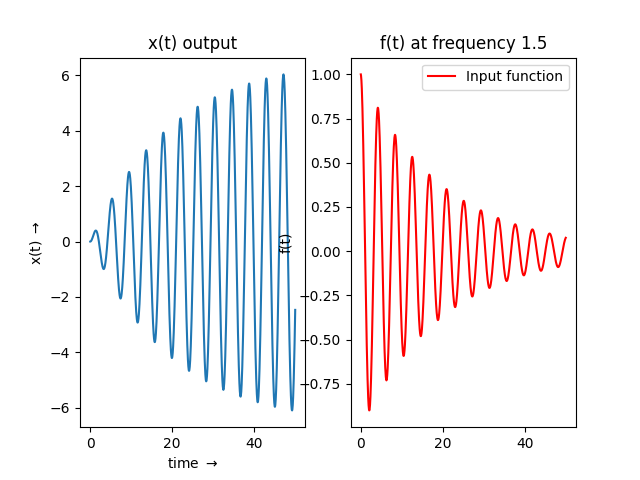
\includegraphics[scale=0.5]{Q3-3.png} 
    \caption{Question 3} 	
    \label{time response q3.3}
   \end{figure} 
   
\begin{figure}[!tbh]
   	\centering
  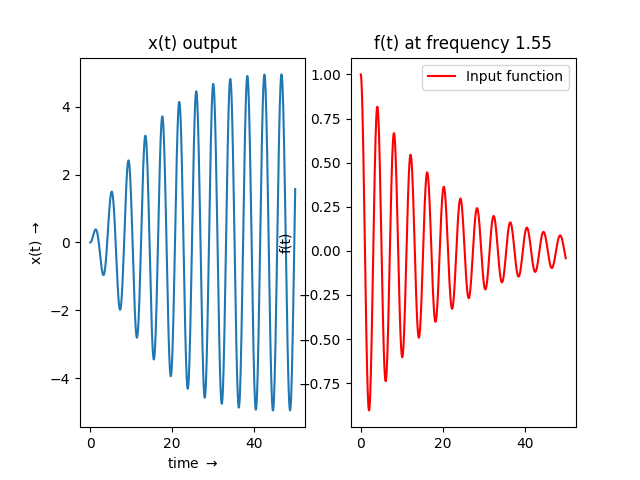
\includegraphics[scale=0.5]{Q3-4.png} 
    \caption{Question 3} 	
    \label{time response q3.4}
   \end{figure} 
   
\begin{figure}[!tbh]
   	\centering
  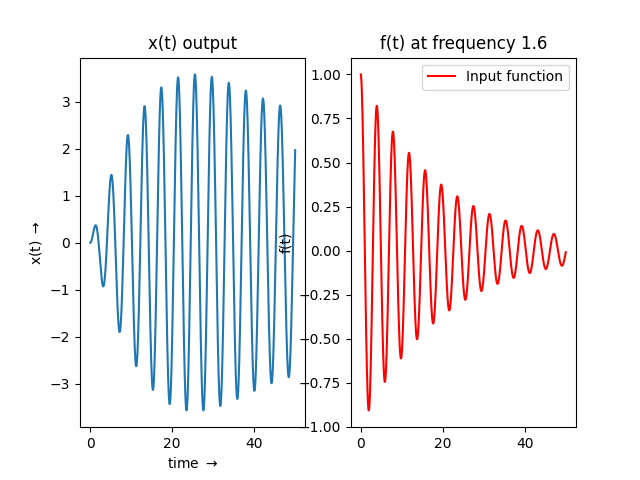
\includegraphics[scale=0.5]{Q3-5.png} 
    \caption{Question 3} 	
    \label{time response q3.5}
   \end{figure} 
   
\subsection{Question 4: Coupled Spring}
$$\frac{d^2x}{dx^2}+(x-y)=0$$
$$\frac{d^2y}{dy^2}+2(y-x)=0$$
given initial conditions $x(0)=1, \dot{x}(0)=y(0)=\dot y(0)=0$. On solving the two equations in Laplace domain, we get
$$X(s)=\frac{s^2+2}{s^3+3s}$$
$$Y(s)=\frac{2}{s^3+3s}$$
Taking inverse and plotting the functions in time domain. 

\begin{verbatim}
X_s_q4 = sp.lti([1,0,2],[1,0,3,0])
t_q4, x_q4 = sp.impulse(X_s_q4,None,np.linspace(0, 20, 100))
plt.plot(t_q4, x_q4,'red')
plt.xlabel('time')
plt.ylabel('x(t)')
plt.title('x(t) - Coupled Spring Problem')
plt.show()

Y_s_q4 = sp.lti([2],[1,0,3,0])
t_q4, y_q4 = sp.impulse(Y_s_q4,None,
  np.linspace(0, 20, 100))
plt.plot(t_q4, y_q4,'red')
plt.xlabel('time')
plt.ylabel('y(t)')
plt.title('y(t) - Coupled Spring Problem')
plt.show()
\end{verbatim}

\begin{figure}[!tbh]
   	\centering
  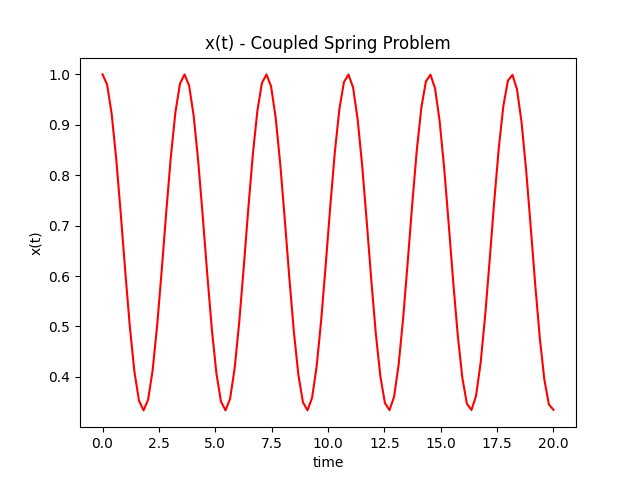
\includegraphics[scale=0.5]{Q4-1.png} 
    \caption{Question 4: $x(t)$} 	
    \label{time response x q4}
   \end{figure} 


\begin{figure}[!tbh]
   	\centering
  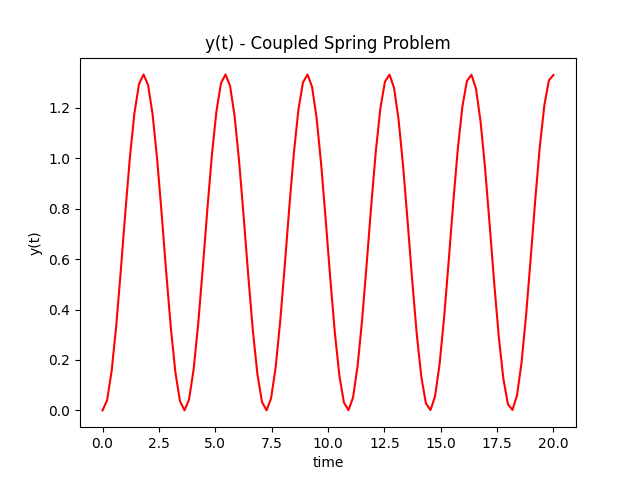
\includegraphics[scale=0.5]{Q4-2.png} 
    \caption{Question 4: $y(t)$} 	
    \label{time response y q4}
   \end{figure} 

\subsection{Question 5: Two Port Network}
The transfer function of the given network is 
$$H(s)=\frac{1}{\frac{s^2}{10^{12}}+\frac{s}{10^{4}}+1}$$
The magnitude and phase response of this function is required. The \texttt{signal} module has a simple way to do this using the method \texttt{bode()} on the transfer function. It returns the frequency, magnitude in decibel scale and the argument. See the following code.

\begin{verbatim}
trans_func = sp.lti([1],[1e-12,1e-4,1])
w,S,phi = trans_func.bode()
\end{verbatim}

Now I have to plot (Figure 10) these to see the variation over frequency.

\begin{verbatim}
plt.subplot(2,1,1)
plt.semilogx(w,S,'red')
plt.title('Magnitude Plot')
plt.xlabel('w (log scale)')
plt.ylabel(r'|H(jw)|_{dB}')
plt.subplot(2,1,2)
plt.semilogx(w,phi)
plt.title('Phase Plot')
plt.xlabel('w (log scale)')
plt.ylabel(r'arg(H(jw))')
plt.show()
\end{verbatim}

\begin{figure}[!tbh]
   	\centering
  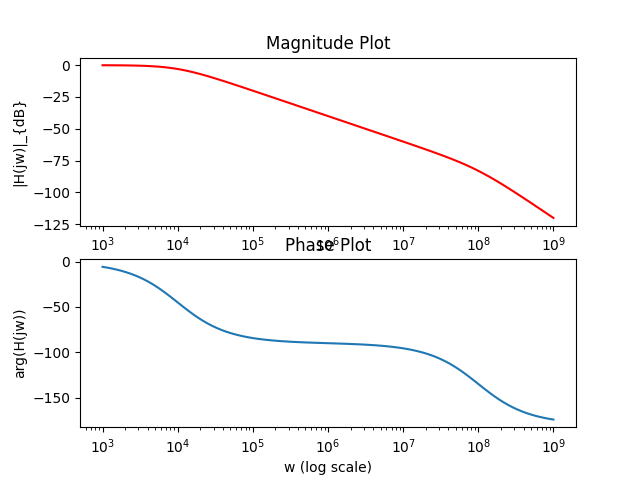
\includegraphics[scale=0.5]{Q5.png} 
    \caption{Magnitude and Phase Plot} 	
    \label{Q5}
   \end{figure} 
   
\subsection{Question 6:}
In the LCR circuit the input signal $$v_i(t)=\cos(10^3)u(t)-\cos(10^6)u(t)$$
$$Vout(t)=Vi(t)*h(t) (convolution)$$
First, we'll see the output signal for first 30 microseconds - the transient. The \texttt{sp.lsim} function takes the transfer function, input signal in time domain and a time array. Here, the higher frequency component decides the behaviour as the $10^3t$ term remains close to zero. 

\begin{verbatim}
t_q6 = np.linspace(0,30e-6,1000)
vin = np.cos(t_q6*1000)-np.cos(t_q6*(10**6))
t_q6,vout,svec = sp.lsim(trans_func,vin,
  np.linspace(0,30e-6,1000))
plt.plot(t_q6,vin,'red',label='Vin')
plt.plot(t_q6,vout,'green',label='Vout')
plt.xlabel('time')
plt.ylabel('voltage')
plt.title('Question 6')
plt.legend()
plt.show()
\end{verbatim}

Then, we'll sketch the output for 10ms, when the system moves towards steady state. The higher frequency component is more or less filtered out and hence, the 1000 rad/sec frequency component is dominant. The  The Figures 11 and 12. 

\begin{verbatim}
t_q6 = np.linspace(0,0.01,1000)
vin = np.cos(t_q6*1000)-    np.cos(t_q6*(10**6))
t_q6,vout,svec = sp.lsim(trans_func,vin,
np.linspace(0,0.01,1000))
plt.plot(t_q6,vin,'red',label='Vin')
plt.plot(t_q6,vout,'green',label='Vout')
plt.xlabel('time')
plt.ylabel('voltage')
plt.title('Question 6')
plt.legend()
plt.show()
\end{verbatim}

\begin{figure}[!tbh]
   	\centering
  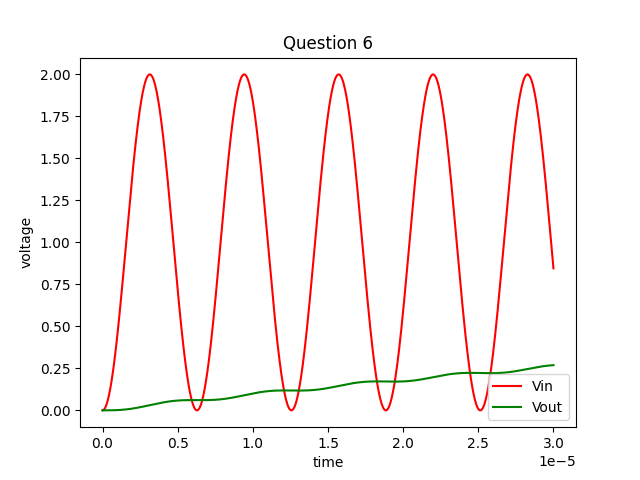
\includegraphics[scale=0.5]{Q6-1.png} 
    \caption{Question 6 - 1} 	
    \label{q6}
   \end{figure} 

\begin{figure}[!tbh]
   	\centering
  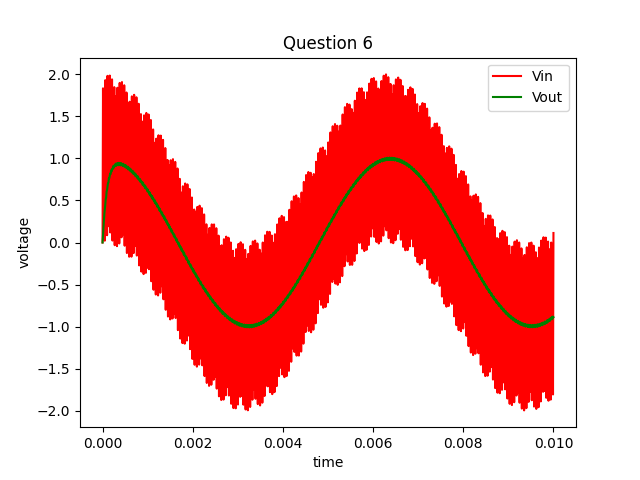
\includegraphics[scale=0.5]{Q6-2.png} 
    \caption{Question 6 - 2} 	
    \label{q6-2}
   \end{figure} 

\section{Conclusion}
The aim that I started the assignment with, is now seen to have been accomplished. The \texttt{scipy.signal} module has super useful functions that make analysis of transfer functions and LTI systems easy. Through this assignment I saw how scientific python can model LTI systems and plot the responses accurately. I saw how forced oscillations, coupled oscillators, and low-pass filters can be analysed. Also I take a moment to appreciate the computing power that can perform millions of operations for getting function values, taking Laplace transforms, for a thousand instants of time and plot that data all in a fraction of a second.   


\end{document}



 